\documentclass[a4paper,12pt]{article}
\usepackage[utf8]{inputenc}

\usepackage[utf8]{inputenc}
\usepackage[T2A]{fontenc}
\usepackage[english,russian]{babel}
\usepackage{amsthm}
\usepackage{amsmath}
\usepackage{amssymb}
\usepackage{tikz}
\usepackage{textcomp}
\usepackage{marvosym}
\usepackage{ esint }
\usepackage{mathtext}
\usepackage{siunitx} % Required for alignment
\usepackage{subfigure}
\usepackage{multirow}
\usepackage{rotating}
\usepackage{afterpage}
\usepackage[arrowdel]{physics}
\usepackage{booktabs}
\setlength{\topmargin}{-0.5in}
\setlength{\textheight}{9.1in}
\setlength{\oddsidemargin}{-0.4in}
\setlength{\evensidemargin}{-0.4in}
\setlength{\textwidth}{7in}
\setlength{\parindent}{0ex}
\setlength{\parskip}{1ex}
\newcommand{\ndiv}{\hspace{-4pt}\not|\hspace{2pt}}
\usepackage{floatrow,graphicx,calc}
\usepackage{float}
\usepackage[export]{adjustbox}
\usepackage{wrapfig}
\usepackage{pgfplots}
\usepackage{caption}
\pgfplotsset{compat=1.16}
\graphicspath{ {./images/} }
\RequirePackage{caption}
\DeclareCaptionLabelSeparator{defffis}{ — }
\captionsetup{justification=centering,labelsep=defffis}
\usepackage{caption} \captionsetup[table]{labelsep=endash,justification=justified,singlelinecheck=false,font=normalsize}
\usepackage{amsfonts,mathtools}

\title{Лабораторная работа № 5.5.1\\Измерение коэффициента ослабления потока $\gamma$-лучей в веществе и определение их энергии}
\author{Илья Прамский}
\date{Октябрь 2024}

\begin{document}
\maketitle
\newpage
\section{Теоретическая справка}
Проходя через вещество, пучок $\gamma$-квантов постепенно ослабляется, ослабление происходит по экспоненциальному закону, который может быть записан в двух эквивалентных формах:
\[\begin{array}{l}
I = I_0 e^{-\mu l} ,\\
I = I_0 e^{-\mu' m_l},\\
\end{array}\]
где $I, I_0$ -- интенсивности прошедшего и падающего излучений, $l$ -- длина пути, пройденного пучком $\gamma$-лучей, $m_l$ -- масса пройденного вещества на единицу площади, $\mu$, $\mu'$ -- константы, зависящие от вещества.\\
Число выбывших на пути $dl$ из пучка $\gamma$-квантов
\[-dN = \mu N dl,\]
откуда
\[N = N_0 e^{\mu l},\]
или
\begin{equation}
\mu = \dfrac{1}{l} \ln \dfrac{N_0}{N}.
\end{equation}

\section*{Описание установки}
\begin{figure}[h]
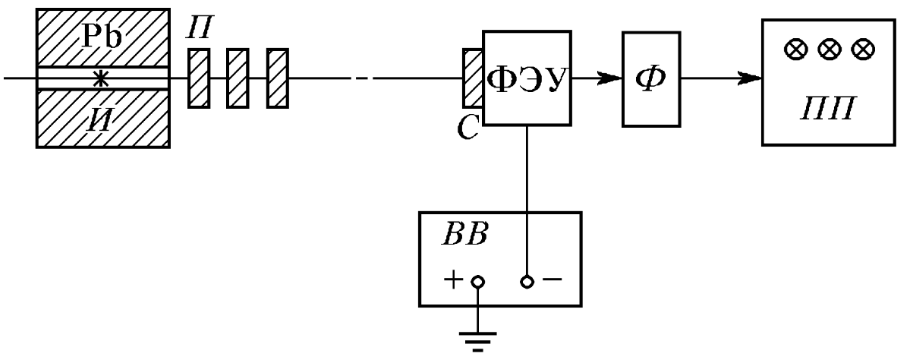
\includegraphics[scale=0.5]{1.png}
\centering
\caption{Схема установки.}
\end{figure}
На Рис. 1 изображена схема установки. Свинцовый коллиматор выделяет узкий почти параллельный пучок $\gamma$-квантов, проходящий через набор поглотителей П и регистрируемый сцинтилляционным счётчиком. Сигналы от счётчика усиливаются и регистрируются пересчётным прибором ПП. Высоковольтный выпрямитель ВВ обеспечивает питание сцинтилляционного счётчика. Чтобы уменьшить влияние плохой геометрии, счётчик расположен на большим расстоянии от источника, поглотители имеют небольшие размеры, а так же устанавливаются на расстоянии друг от друга, чтобы испытавшие комптоновское рассеяние кванты с меньшей вероятностью могли в него вернуться.

\section*{Ход работы}
Число поглощаемых частиц при отсутствии заглушки
\[N_0 = 19680 \pm 40 \]

Число поглощаемых частиц в присутствии поглотителя(фон)
\[N_\text{фон} = 18\]

В дальнейшем за $N_0$ примем число, равное $N_0 - N_\text{фон}$, а также у всех измерений будем вычитать $N_\text{фон}$.

$\sigma_l = 0,01$ см

\begin{table}[H]
\centering
\begin{tabular}{|c|c|c|c|c|c|c|c|c|}
\hline
\multicolumn{3}{|c|}{Свинец} & \multicolumn{3}{|c|}{Железо} & \multicolumn{3}{|c|}{Алюминий} \\
\hline
\multicolumn{3}{|c|}{$l_0 = 0,50$ см} & \multicolumn{3}{|c|}{$l_0 = 1,00$ см} & \multicolumn{3}{|c|}{$2,00$ см} \\
\hline
$N_\text{пластин}$ & $N_\text{част}$ & $\sigma_{N_\text{част}}$ & $N_\text{пластин}$ & $N_\text{част}$ & $\sigma_{N_\text{част}}$ & $N_\text{пластин}$ & $N_\text{част}$ & $\sigma_{N_\text{част}}$ \\
\hline
1 & 10880 & 40 & 1 & 11160 & 40 & 1 & 12980 & 40 \\
\hline
2 & 6130  & 30 & 2 & 6260 & 30 & 2 & 8580 & 30 \\
\hline
3 & 3510  & 20 & 3 & 3490 & 20 & 3 & 5690 & 20  \\
\hline
4 & 2040  & 10 & 4 & 2000 & 10 & 4 & 3820 & 20  \\
\hline
5 & 1240  & 10 & 5 & 1158 & 9 & 5 & 2530 & 20 \\
\hline
6 & 750   & 6  & 6 & 669 & 6 & 6 & 1720 & 10 \\
\hline
7 & 505   & 5  & 7 & 405 & 4 &   & &       \\
\hline
8 & 361   & 4  & 8 & 251 & 3 &   & & \\
\hline
9 & 256   & 3  &   &     &   &   & & \\
\hline
10 &217  & 2  &    &     &   &   & & \\
\hline
\end{tabular}
\end{table}

\newpage
Преобразуем формулу для коэффициента ослабления
\[\ln(N) = -\mu l + \ln(N_0)\]

Тогда получается график зависимости $ln(N)$ от $l$

\begin{figure}[H]
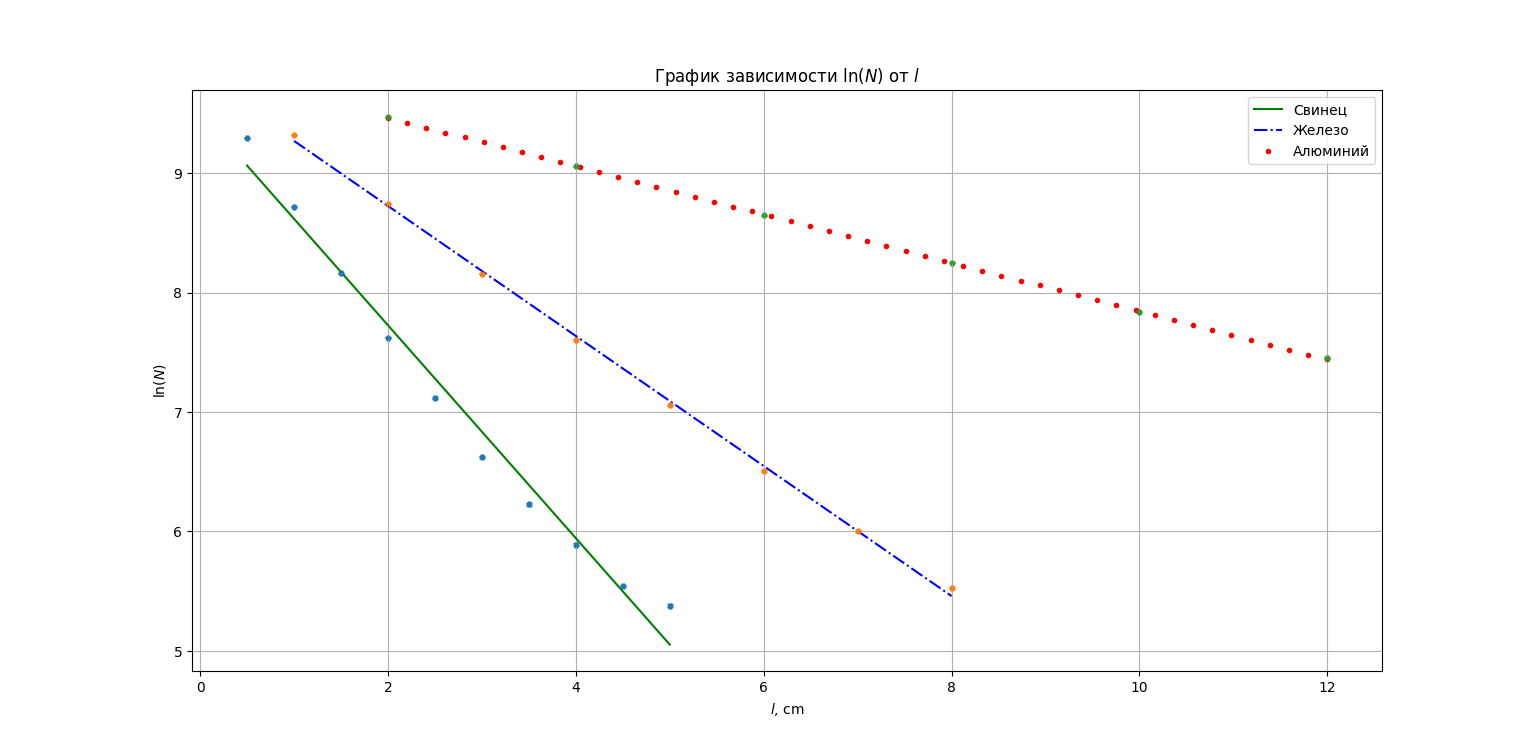
\includegraphics[scale=0.5]{graph.png}
\end{figure}

\begin{figure}[H]
\centering
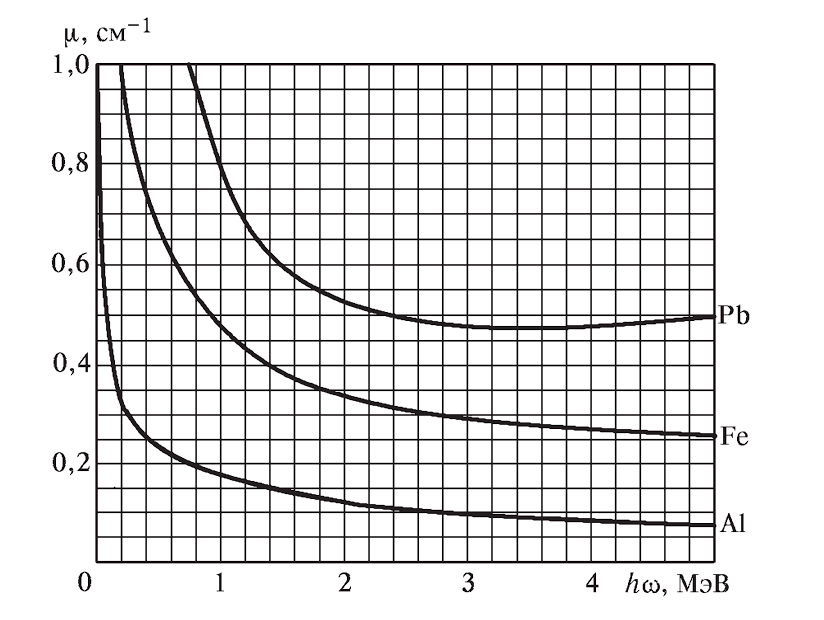
\includegraphics[scale=0.5]{graph1.png}
\end{figure}

\begin{table}[H]
\begin{tabular}{|c|c|c|c|}
\hline
Материал & $\mu, 10^{-3} \text{см}^{-1}$ & $\sigma_\mu,10^{-3} \text{см}^{-1}$ & $<\varepsilon>$, МэВ \\
\hline
Свинец & $890$ & $20$ & 0,84\\
\hline
Железо & $544$ & $7$ & 0,83\\
\hline
Алюминий & $202$ & $1$ & 0,77\\
\hline
\end{tabular}
\end{table}

\section*{Вывод}
В ходе работы был вычислен коэффициент ослабления потока $\gamma$ - лучей в веществе, также была вычислена средняя энергия $\gamma$-лучей.

\end{document}